\chapter{Contribuições do feminismo para a compreensão e intervenção em casos de relacionamento abusivo}\sectionmark{Contribuições do feminismo para a compreensão e intervenção em casos de relacionamento abusivo}
\begin{flushright}
\begin{scriptsize}
    Analu Ianik Costa
\end{scriptsize}
\vspace{1cm}
\end{flushright}

A violência contra a mulher perpetrada por parceiros íntimos é um problema de saúde pública recorrente em diversos países. De acordo com a Organização Mundial da Saúde (OMS), o índice de mulheres entre 15 e 49 anos vítimas deste tipo de violência pode chegar a 69\% (WHO, 2014). A violência contra a mulher caracteriza-se:

\begin{quote}
    ``pela intenção do marido ou companheiro de intimidar, seja por ameaça ou pelo uso da força física à mulher ou a algo de sua propriedade. O propósito final da agressão é controlar o comportamento da mulher por meio da indução de medo. Subjacente a todo tipo de abuso está um desequilíbrio nas relações de poder entre a vítima e o agressor.'' (Sinclair, 2010 p 73)
\end{quote}

O Mapa da Violência, divulgado em 2012, traz dados sobre o aumento de assassinato de mulheres no Brasil entre os anos de 1980 e 2010. Uma comparação entre o número de homicídios ocorrido no ano de 1990 e no ano de 2010 aponta um aumento de 230\% neste índice. Segundo a OMS, o Brasil é o sétimo colocado com relação ao índice de homicídios contra mulheres, com uma taxa de 4,4 homicídios por ano para cada 100 mil mulheres. Os percentuais de violência se dividem em: física (44,2\%), psicológica (acima de 20\%) e sexual (12,2\%) (Waiselfisz, 2012). De acordo com Day et al. (2003), a agressão física dificilmente ocorre de uma maneira isolada, sendo quase sempre acompanhada de violência psicológica e, em 25 a 50\% dos casos, de violência sexual.

Segundo o IPEA (Instituto de Pesquisa Econômica Aplicada), 40\% das mulheres são assassinadas pelos seus parceiros ou ex-parceiros. No Brasil, cerca de 29\% dos feminicídios aconteceram no domicílio da vítima, 31\% em via pública e 25\% em ambientes de saúde. No período entre 2009 e 2011, foram registrados 13.071 feminicídios, o equivalente a cerca de 427 mulheres mortas a cada mês, em média 15 por dia (Sant’anna e Penso, 2015).

Os dados apresentados acima sobre violência contra a mulher praticada por parceiros ou ex-parceiros são alarmantes. Esta alta incidência mundial levanta questionamentos como: Quais fatores individuais estão envolvidos em relacionamentos abusivos? Quais variáveis culturais contribuem para este alto índice? E principalmente: enquanto terapeutas, o que podemos fazer sobre isso?

O objetivo deste capítulo é discutir aspectos teóricos sobre relacionamentos abusivos e aplicá-los a um estudo de caso, apresentando ainda possibilidades de intervenção, considerando que este problema social está relacionado a um cenário cultural complexo de opressão a mulher. Para isso, a intervenção é pautada na Análise do Comportamento, mais especificamente na Terapia Feminista e na Psicoterapia Analítica Funcional com um viés feminista.

A intersecção entre a Psicologia e o Feminismo resulta na Psicologia Feminista, que se afirma enquanto resposta a um modelo de ciência positivista e androcêntrica que, ao se considerar neutra e tradicional, desconsidera o contexto cultural, social e político. A psicologia feminista, portanto, abarca a influência de variáveis socioculturais aos aspectos psicológicos relacionados à violência de gênero, que se acredita estar diretamente relacionada à violência contra a mulher (Farias \& Castro, 2016). 

Ao adotar um viés feminista da compreensão do fenômeno e de possibilidades de intervenção com as vítimas de violência, os psicólogos exploram também a perspectiva de contribuir para uma transformação social, na medida em que o cerne da terapia feminista é justamente conectar as demandas trabalhadas na terapia com questões políticas - neste caso, de opressão a mulher - e construir assim o caminho para uma importante mudança nas práticas culturais patriarcais.

\section{Relacionamento abusivo}

Para compreender a dinâmica do relacionamento abusivo, é necessário discutir aspectos culturais e o conjunto de processos que tem na sua base o sexismo e o patriarcado como formas de organização social. Uma vez que os papéis sociais são distribuídos de acordo com gênero, e essa segregação ocorre muitas vezes de maneira velada. A desigualdade salarial apontada pela Catho\footnote{\url{https://tinyurl.com/feminismo100}} explicita que, independente do cargo, a mulher recebe menos que o homem, e que uma vez que a mulher se torna mãe essa diferença tende a aumentar ainda mais de acordo com o número de filhos. O mesmo não acontece com homens que são pais. Isto configura uma violência social de gênero que precede a agressão entre os parceiros na medida em que coloca a mulher à margem de constructos sociais. A maneira patriarcal que a sociedade se estabelece privilegia a experiência masculina enquanto a feminina é desvalorizada e negligenciada, conforme ressaltado pelos dados apresentados sobre as diferenças profissionais entre homens e mulheres (Narvaz \& Koller, 2006).

A assimetria de gêneros está na base do relacionamento abusivo. É importante diferenciar os conceitos de sexo e gênero. O sexo corresponde à identidade biológica, em diferenciar os seres nas categorias macho e fêmea, enquanto o gênero refere-se a comportamentos socialmente aprendidos diante das expectativas da cultura que estamos inseridos (Dias \& Machado, 2008). ``As diferenças de gênero são entendidas como descrições modeladas pelos padrões culturais, não devem ser aceitas como naturais e devem ser alvo de uma análise crítica.'' (Dias \& Machado, 2008, p. 573) 

Estes comportamentos variam e estão associados a cada um dos sexos, portanto a dimensão que os seleciona é cultural e não biológica, apesar dos esforços de algumas correntes teóricas em apontar diferenças estruturais no cérebro de homens e mulheres e utilizá-las como justificativa da instabilidade emocional feminina, por exemplo, e para que o papel da mulher na sociedade fosse restringido à mãe e esposa.

Verifica-se uma assimetria sistemática de gênero à medida que se propaga a ideia da superioridade e dominância do masculino perante o feminino. A construção social que coloca o corpo feminino visto como mais violável e fraco, coloca a mulher como socialmente e sexualmente vulnerável. A partir do momento que o masculino é enfatizado como dominante, é exercido um controle sobre a mulher que a coloca em um ciclo no qual ela cada vez mais é convencida da sua fraqueza e recai em situaçõesde vitimização (Dias \& Machado, 2008).

Cortez e Souza (2008) destacam que a questão da manutenção dos padrões tradicionais de gênero por meio da preservação de uma estrutura familiar patriarcal aparece como base importante para a compreensão dos conflitos domésticos e das agressões dos maridos contra suas esposas. Ao analisar entrevistas realizadas com mulheres vítimas de violência doméstica, observaram que os valores tradicionais que são relacionados aos papéis atribuídos culturalmente ao homem e à mulher predominam (e.g., a visão do homem como provedor e protetor da família, como alguém que deve ocupar o espaço público e com o seu trabalho garantir meios para a subsistência familiar, enquanto a mulher tem mais valor desempenhando o seu trabalho no espaço privado).

Percebe-se como a perpetuação desses papéis socialmente construídos influencia na vitimização feminina. Quando é imposta à mulher a restrição de ocupar apenas espaços privados, ela é sentenciada a viver a violência sem poder contar com o amparo devido que é proporcionado apenas pelos espaços públicos - ou pelos menos deveria, mas sabe-se que essa rede de proteção deixa a desejar, como no caso de Gravelina, que denunciou o ex-marido, relatou as ameaças e agressões prévias, comprovadas com exames de corpo e delito, porém nada foi feito pelos órgãos responsáveis e no mesmo dia que procurou ajuda (depois de tentativas anteriores) ela foi assassinada brutalmente pelo ex, denotando uma falha em toda a rede de apoio que deveria proteger a mulher vítima de violência doméstica (Williams, 2001).

O papel da mantenedora do equilíbrio emocional do relacionamento, priorizando a honestidade e a fidelidade, que é atribuído à mulher, nada mais é do que um controle social que valida o poder do homem sobre ela (Sant’anna \& Penso, 2015). Tendo em vista que cabe à mulher toda a responsabilidade emocional do relacionamento, ela acaba atarefada com mais uma função invisível que desempenha. Essa sobrecarga reflete na sua saúde mental e também pode influenciar o seu desempenho profissional e social, atuando dessa forma como um mecanismo de controle. 

A valorização do sacrifício da mulher em nome do bem-estar dos filhos e da preservação da instituição familiar (Cortez \& Souza, 2008) é outra face deste controle. A responsabilização da mulher pela harmonia no lar, pela educação dos filhos e satisfação conjugal corrobora a visão que, se ela está sendo vítima de violência doméstica, provavelmente é porque falhou na sua missão de construir um lar onde prevalecem os valores familiares.

Bell e Naugle (2005) apontam que, quanto mais a mulher investe afetivamente no casamento/namoro, mais ela acredita que esta relação deve ser preservada. Em um relacionamento abusivo, a mulher tende a supor que a responsabilidade de fazer as agressões cessarem é dela e que se elas continuam é porque ela não está se dedicando o suficiente, então ela passa a doar-se mais. Outro fator determinante no investimento que a mulher faz na relação é que, devido à intermitência das agressões, ela tem esperança que estas acabem e ela possa usufruir da ``parte boa'' do companheiro. Porém, segundo as autoras, quanto maior é esta movimentação em direção a construir uma relação saudável, mais aprisionada a mulher se sente ao parceiro.

\begin{figure}[h]
    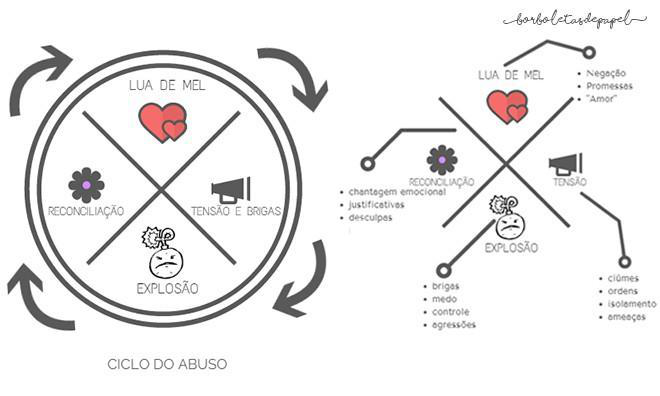
\includegraphics[width=1\textwidth]{10/figura1.png}
    \captionof{figure}{Representação do ciclo da violência em relacionamentos abusivos. Fonte: \url{https://tinyurl.com/feminismo100}}
\end{figure}

O ciclo apresentado acima conta com quatro fases, sendo elas: tensão e brigas, explosão, reconciliação e lua de mel. Cada fase tem suas características, podendo variar a intensidade e topografia dos comportamentos.

A fase de tensão e brigas é caracterizada quando o homem, por meio do controle que exerce sobre a mulher, ciúme excessivo, manipulação e o isolamento social compulsório; cria um ambiente tenso no qual as brigas se tornam frequentes e a mulher fica sob uma extrema pressão, apresentando picos de ansiedade. Nesta fase a mulher busca agir de forma a evitar a próxima fase, que será a da agressão. Ormeno \& Cortiano (2016) apontam que estilos parentais, os maus tratos vivenciados e a ansiedade da família de origem do agressor são determinantes para a perpetração deste modelo de violência. O uso de álcool ou outras substâncias ilícitas são desencadeadores, e não causadores da violência.

Porém, um fato que endossa a visão feminista do relacionamento abusivo é o direcionamento das agressões. A partir do momento que homens com padrão comportamental violento agridem apenas as suas parceiras íntimas e não o fazem com mais ninguém, identifica-se a assimetria de poder como fulcral no cometimento das agressões. Segundo Murta, Ramos, Tavares, Cangussú \& Costa (2014), a agressão contra a mulher companheira é algo aprendido e que está relacionado à utilização da agressividade para a resolução de conflitos, à banalização da violência de gênero e aos amigos que endossam a violência.

A fase da explosão é quando a agressão ocorre. Esta agressão pode ser física ou sexual. Sabe-se que essas formas de violência também são acompanhadas pela violência psicológica, porém o abuso psicológico já está presente na fase de tensão, não sendo exclusivo da fase de explosão. A incontrolabilidade das agressões, aliada a um discurso culpabilizador do parceiro - que ecoa julgamentos de toda a sociedade -, faz com que a mulher acredite que é a culpada pela violência que vem sofrendo. Bell e Naugle (2005) afirmam que o desamparo aprendido é um dos fatores que impedem a saída da mulher desse relacionamento abusivo. Diversas tentativas são feitas no intuito de minimizar ou encerrar as agressões, porém dificilmente estas são efetivas. Para trabalhar o desamparo aprendido, as autoras ressaltam a importância do afastamento da mulher, pois isso vai fazer com que elas percebam a culpabilização imposta e outros aspectos importantes da dinâmica do relacionamento, aumentando a probabilidade da mulher concretizar o término.

Após a ocorrência da agressão, que é o ápice da fase da explosão, vem a fase da reconciliação. Nesta fase, o companheiro agressor busca se reaproximar da mulher para manter a relação. Frequentemente ele apresenta comportamentos de arrependimento (há dúvidas sobre o quão genuíno é este sentimento), chantagem emocional e variabilidade comportamental para conquistar o perdão da parceira.

É neste período da reconciliação que a intervenção psicoterápica tem uma maior chance de ser eficaz. Quando a mulher se afasta e acaba com qualquer contato que tem com o agressor, menores são as chances das manipulações e do controle exercidos por ele serem bem-sucedidos, e isto aumenta a efetividade da intervenção.

Por fim, tem-se a fase da lua de mel, que segue a reconciliação e é o momento em que o controle volta a ser exercido, porém com a utilização do reforçamento positivo. Nesta fase o homem investe em comportamentos românticos em sua topografia, mas que seguem no intuito do controle. A mulher nem sempre acredita que o companheiro vai deixar de agredi-la e que essa fase irá durar, porém saber que as agressões cessarão, mesmo que temporariamente é altamente reforçador para ela.

De acordo com Perone (2003), o controle nem sempre é feito utilizando a coerção. Além da punição e dos esquemas de reforçamento negativo, é possível também fazê-lo empregando o reforçamento positivo. Segundo o autor, o reforço positivo também pode apresentar consequências aversivas, porém frequentemente elas se apresentam com um atraso. A partir do momento que o agressor faz o controle por meio do reforçamento positivo, ele elimina momentaneamente o aspecto aversivo deste, diminuindo assim a chance da parceira engajar-se em comportamentos de contracontrole.

É justamente devido à configuração deste ciclo de violência que é comum que a mulher tenha sentimentos ambivalentes com relação ao homem que perpetrou as agressões. A alternância entre as fases e a modificação do comportamento do parceiro configuram um esquema de reforçamento intermitente, e a raiva e o medo alternam com sentimentos de alívio que podem ser confundidos com amor e desejo de proximidade da mulher com o parceiro.

\section{Terapia feminista}

O viés feminista está presente em algumas abordagens de psicoterapia. Na década de 70, algumas mulheres terapeutas familiares sistêmicas se uniram e fundaram o ``\textit{Women’s Institute for Life Studies}''. O objetivo do instituto era produzir pesquisas na área da terapia familiar sistêmica, porém abarcando os temas relacionados ao movimento feminista. Foram propostas mudanças na maneira de compreender a dinâmica familiar, e os papéis atribuídos socialmente ao marido e à esposa, à mãe e ao pai, passaram a ser considerados na formulação dos casos e nas intervenções propostas. Esta nova forma de pensar o processo terapêutico foi chamada de terapia feminista da família (Sant’anna \& Penso, 2015). 

As correntes da terapia feminista atribuem a dominação masculina à gênese das desigualdades de gênero. Uma das consequências diretas dessa dominação é a dinâmica das relações violentas das quais as mulheres são vítimas (Narvaz \& Koller, 2006), considerando as estatísticas apresentadas inicialmente sobre violência contra a mulher. 

Além da terapia feminista da família, as autoras Neves, Cunha, Grangeia e Correia (2015) propuseram um grupo feminista de reflexão e ação para intervir com mulheres vítimas de violência na intimidade. Os objetivos do grupo são: 1) informar sobre o fenômeno da violência de gênero, 2) desconstruir discursos de gênero, 3) refletir em torno dos significados e dos impactos das histórias pessoais de vitimização e 4) promover o \textit{empowerment} - empoderamento\footnote{Para uma explanação sobre o conceito de empoderamento, ver capítulo 06.} - e a capacitação pessoal e social. Percebe-se que a discussão de variáveis machistas que contribuem para a violência de gênero é o ponto inicial determinante para a efetividade das próximas etapas de autoconhecimento, fortalecimento pessoal e desenvolvimento de autonomia.

Ao utilizar uma visão da psicologia clínica feminista, o objetivo é que a terapeuta esteja consciente da desigualdade na relação de poder entre ele e a cliente. Por serem humanos, que cresceram em uma sociedade patriarcal, terapeutas podem engajar-se em comportamentos que reproduzem relações de poder e privilégio (Terry, Bolling, Ruiz \& Brown, 2010). A partir do momento que essa diferença é reconhecida, o terapeuta deve estar atento para não reproduzir no ambiente da terapia os mesmos mecanismos de opressão aos que a cliente está sujeita. 

\section{Psicoterapia Analítica Funcional e feminismo}

A Psicoterapia Analítica Funcional – FAP, proposta por Kohlenberg e Tsai (1991) trabalha com os comportamentos-problema dos clientes que ocorrem na sessão, chamados de CCR1 (comportamento clinicamente relevante 1), os progressos dos clientes que ocorrem na sessão, CCR2 (comportamento clinicamente relevante 2) por entender que esses comportamentos que ocorrem na interação com a terapeuta são semelhantes ao que os clientes emitem em seu contexto social.

Porém, ``a terapia será ineficaz caso o cliente melhore no ambiente terapêutico, mas esses ganhos não se transfiram para a vida cotidiana'' (Kohlenberg \& Tsai, 2001, p. 17); logo cabe ao terapeuta facilitar a habilidade de generalização da cliente, para que ele possa reproduzir o modelo positivo aprendido na terapia em outros contextos nos quais ela está inserida. Na medida em que o cliente passa a compreender quais são os estímulos reforçadores, eliciadores e discriminativos (CCR3) relacionados aos seus comportamentos ele os modifica dentro e fora da sessão, demonstrando generalização.

As ações da terapeuta feminista que utiliza a FAP visam não apenas auxiliar a cliente na sua demanda, como também mobilizá-la para praticar uma mudança social. Acredita-se que este engajamento tem um papel terapêutico fundamental. As autoras Terry et al. (2010) recomendam estes cinco passos para a aproximação do terapeuta a variáveis socioculturais e à consolidação de uma prática clínica feminista: 

\begin{enumerate}
    \item Identificar e avaliar a importância da posição social do cliente (etnia, gênero, classe social, orientação sexual);
    \item Comportamentos do cliente como estratégias para lidar com ambientes não saudáveis ou opressores (comportamento de contracontrole);
    \item Análise dos papéis de gênero, cultura e relações de poder;
    \item Encorajar clientes a começarem uma mudança social; e
    \item Terapeuta também ter uma iniciativa de mudança social
\end{enumerate}

Para a formulação do caso, Terry et al. (2010) propuseram um modelo no qual, além dos comportamentos-problema e alvos do cliente (CCR1 e CCR2), também são avaliados os SP1 (Sociopolítico 1), que seriam os comportamentos do cliente ou do terapeuta que ocorrem em sessão e que reforçam ou mantêm relações de poder e privilégio baseadas na participação individual de um grupo social específico. Já os SP2 (sociopolítico 2) seriam os comportamentos de melhora do cliente e do terapeuta em sessão, relacionados a não reproduzir relações de poder em terapia.

Para a formulação do caso, Terry et al. (2010) propuseram um modelo no qual, além dos comportamentos-problema e alvos do cliente (CCR1 e CCR2), também são avaliados os SP1 (Sociopolítico 1), que seriam os comportamentos do cliente ou do terapeuta que ocorrem em sessão e que reforçam ou mantêm relações de poder e privilégio baseadas na participação individual de um grupo social específico. Já os SP2 (sociopolítico 2) seriam os comportamentos de melhora do cliente e do terapeuta em sessão, relacionados a não reproduzir relações de poder em terapia.

% Please add the following required packages to your document preamble:
% \usepackage{booktabs}
% \usepackage{graphicx}
\begin{table}[h]
    \caption{My caption}
    \label{tabela1}
    \resizebox{\textwidth}{!}{%
    \begin{tabular}{@{}lll@{}}
    \toprule
    \textbf{Característica cultural}                                                                                           & \textbf{Poder}                                                                             & \textbf{Menos poder}                                                                                                                                                \\ \midrule
    A - Idade (age)                                                                                                            & Adultos                                                                                    & Crianças, adolescentes e idosos                                                                                                                                     \\
    \begin{tabular}[c]{@{}l@{}}D - Necessidades especiais\\ (developmental disabilities)\end{tabular}                          & Pessoas aptas fisicamente                                                                  & \begin{tabular}[c]{@{}l@{}}Indivíduos portadores de\\ necessidades especiais\end{tabular}                                                                           \\
    \begin{tabular}[c]{@{}l@{}}D - Deficiência adquirida\\ ao longo da vida\\ (disability acquired later in life)\end{tabular} & Pessoas aptas fisicamente                                                                  & \begin{tabular}[c]{@{}l@{}}Indivíduos que adquiriram alguma\\ condição ao longo da vida\end{tabular}                                                                \\
    R - Religião (religion)                                                                                                    & Cristãos (católicos)*                                                                      & Não católicos                                                                                                                                                       \\
    E - Etnia (ethnicity)                                                                                                      & Brancos ou caucasianos                                                                     & Demais etnias                                                                                                                                                       \\
    \begin{tabular}[c]{@{}l@{}}S - Status econômico\\ (socioeconomic status)\end{tabular}                                      & \begin{tabular}[c]{@{}l@{}}Ricos e classe média\\ (acesso ao ensino superior)\end{tabular} & \begin{tabular}[c]{@{}l@{}}Pessoas com um status menor \\ devido a sua ocupação, educação,\\ rendimentos ou origem e/ou \\ habitação em ambiente rural\end{tabular} \\
    \begin{tabular}[c]{@{}l@{}}S - Orientação sexual\\ (sexual orientation)\end{tabular}                                       & Heterossexuais                                                                             & Gays, lésbicas e bissexuais                                                                                                                                         \\
    \begin{tabular}[c]{@{}l@{}}I - Ascendência indígena\\ (indigenous heritage)\end{tabular}                                   & Não indígenas                                                                              & Indígenas                                                                                                                                                           \\
    \begin{tabular}[c]{@{}l@{}}N - Nacionalidade\\ (national origin)\end{tabular}                                              & Estadunidenses**                                                                           & \begin{tabular}[c]{@{}l@{}}Imigrantes, refugiados e\\ intercambistas\end{tabular}                                                                                   \\
    G - Gênero (gender)                                                                                                        & Masculino                                                                                  & \begin{tabular}[c]{@{}l@{}}Feminino, transgênero e\\ pessoas intersexuais\end{tabular}                                                                              \\ \bottomrule
    \end{tabular}%
    }
    \caption*{* Deve-se observar qual é a religião que detém mais poder no país do terapeuta e cliente.\\** Como o modelo foi desenvolvido nos Estados Unidos, a nacionalidade com maior poder é a estadunidense. Deve-se adaptar essa seção à nacionalidade do país aonde a terapia vem sendo conduzida. Assim como é importante adaptar todas as categorias que detém mais poder de acordo com o país onde estão o terapeuta e o cliente.
    }
    \end{table}

Os SP1 e 2 são separados em classes e suas iniciais em inglês formam o acrônimo ADDRESSING, com o intuito de facilitar a lembrança de todas as variáveis sociopolíticas que podem impactar a vida do cliente e do terapeuta (Tabela \ref{tabela1}).

Segundo Fideles e Vandenbergue (2014):

\begin{quote}
    Quando há atenção declarada nos valores pessoais e no aumento de consciência social de cliente e terapeuta, fala-se em Green FAP (expressão derivada do movimento verde). Esta parte do pressuposto de que a consciência social e ecológica tanto auxilia os objetivos individuais dos clientes quanto beneficia a comunidade de uma maneira mais ampla (p.21).
\end{quote}

O terapeuta pode, portanto, ao fazer o contrato da terapia, informar ao cliente que, além de trabalhar problemas e objetivos individuais em terapia, incluirá questões sociopolíticas e questões mais abrangentes da sociedade. Quando o foco de trabalho é com a Green FAP, o terapeuta não só pode como deve trazer seus valores de justiça social para dentro da sessão.

\section{Estratégias psicoterápicas}

Nesta seção, será apresentado um estudo de caso com o objetivo de traçar paralelos entre a teoria apresentada anteriormente e as possibilidades de atuação da terapeuta feminista frente a situações de relacionamento abusivo. As terapias feministas têm como foco, entre outras coisas, auxiliar as mulheres vítimas de violência a desenvolver um repertório comportamental de enfrentamento diante das agressões sofridas. Sensibilizar a cliente para a importância da união feminina e a criação de uma rede de apoio são fundamentais para alcançar o objetivo de mudança social almejado.

\subsection{Identificação da cliente}

Fernanda (nome fictício), 21 anos, estudante universitária, no momento que buscou a terapia estava desempregada. Mora com os pais e o irmão mais velho. Tem uma boa rede social, com amizades de infância preservadas. 

\subsection{Queixa inicial}

Fernanda procurou terapia pois havia terminado um relacionamento abusivo há 2 dias. Relatou que já há algum tempo pensava em terminar o namoro, pois nunca havia sido feliz no relacionamento, uma vez que desde o início percebia as chantagens emocionais praticadas pelo ex. O comportamento dele foi ficando cada vez mais agressivo desde a manipulação, agressão verbal e física. Fernanda relata que, sempre que as agressões se intensificavam, ela tentava se afastar, mas ele ameaçava suicídio ou agredi-la ainda mais. Neste período, imediatamente após o término, ela encontrava-se deprimida, ansiosa e com indicativos de transtorno do estresse pós-traumático. 

\subsection{Relato do relacionamento}

Henrique conheceu Fernanda, se interessou por ela e começou a chamá-la para sair, se aproximar dos amigos e amigas dela e frequentar lugares onde poderia encontrá-la. Em um churrasco eles ficaram, porém Fernanda disse na ocasião que não estava à procura de nada sério. A insistência por parte dele começou a aumentar e ela cedeu, iniciando o relacionamento.

Fernanda relata que, após a oficialização do relacionamento, ela sentiu mudanças no comportamento de Henrique. Inicialmente ele começou a tratá-la grosseiramente, sob o pretexto de sobrecarga no trabalho. Manifestações de ciúme e controle também começaram a acontecer. Ele a telefonava cerca de 3 vezes ao dia dizendo que estava com saudades, questionando o que ela estava fazendo - inicialmente Fernanda entendia essas ligações como manifestações de carinho e uma tentativa de manter uma proximidade saudável - e também começou a interferir na proximidade dela com alguns amigos. Essas atitudes começaram a incomodá-la e ela decidiu conversar com ele sobre e então ele passou a agredi-la verbalmente, dizendo que ela estava exagerando, que toda menina gostaria de um namorado atencioso, carinhoso e que ficasse próximo assim como ele. Percebe-se que a todo momento Henrique invalida as percepções e sentimentos de Fernanda e inverte a situação para que ela seja a culpada das brigas do casal.

A cliente relatou que após um período houve a primeira agressão física: ele pegou-a pelos ombros e apertou, demonstrando descontentamento pelas queixas trazidas por ela sobre o seu comportamento grosseiro e possessivo. A partir destes episódios, Fernanda passou a cogitar terminar o relacionamento, porém, sempre que ele percebia o afastamento dela, ele a manipulava falando que iria mudar, que era uma fase ruim e apresentava diversas atitudes românticas em sua topografia com a função de controle.

Foi se estabelecendo esse padrão das fases do relacionamento abusivo, no qual eles passavam por um período de tensão que culminava na agressão, então ele se mostrava arrependido, acontecia a reconciliação e, por fim, na fase da lua de mel, os dois passavam por momentos ``bons''. Na medida em que um novo ciclo iniciava e se completava, as agressões entraram em escalada e se tornavam cada vez mais graves. Fernanda tinha vergonha de contar para as pessoas sobre o que estava acontecendo por acreditar que a culpa era sua e que seria julgada, uma vez que Henrique mantinha um bom relacionamento com a rede de apoio dela, no intuito de descredibilizar os relatos dela sobre as agressões sofridas. 

Considerando que não cabe à terapeuta atuar com a sua cliente de modo a convencê-la a terminar o relacionamento definitivamente, é importante discutir qual seria então o seu papel e, principalmente, quais seriam as estratégias mais efetivas para proteger mulheres vítimas de violência. Segundo Williams (2001), o terapeuta deve direcionar a cliente a chegar à conclusão que a violência é inaceitável e insustentável em qualquer tipo de relacionamento. Além disso, deve ensinar à cliente sobre quais são os efeitos do controle coercitivo a que ela está exposta e também analisar as sequelas observadas em crianças que residem em lares violentos (Williams, 2001).

O ensino de técnicas de contracontrole também é essencial, desenvolvendo um repertório de enfrentamento que não consiste em tornar-se agressiva ou utilizar os mesmos subterfúgios empregados pelo parceiro, pois isso pode aumentar a gravidade das agressões praticadas por ele. O intuito é deixar a vítima mais preparada e menos passiva às agressões cometidas pelo seu parceiro violento (Williams, 2001), para isso o terapeuta pode auxiliá-la a perceber quais são os comportamentos dela que podem desencadear a agressão. Esta estratégia tem o intuito unicamente de proteger a mulher de futuras agressões e não de culpabilizá-la, pois cabe apenas ao agressor a responsabilidade pela violência.

Cabe ao terapeuta também identificar se a cliente apresenta indicativos de depressão, uma vez que esta é uma das consequências do relacionamento abusivo (Ormeno \& Cortiano, 2016) este dado também pode ser de grande valia para quando a cliente não traz a queixa de relacionamento abusivo, porém aparenta estar deprimida, e então o terapeuta deve investigar qual é o status atual de relacionamento e se a cliente está sendo vítima de violência por parte do parceiro íntimo.

É importante que a terapeuta conheça a dinâmica do relacionamento abusivo e as suas fases, pois desta forma pode compreender funcionalmente as atitudes que o homem apresenta após o término. No caso de Fernanda, passados alguns dias do término do relacionamento, Henrique fez uma surpresa que pode ser considerada romântica, se analisarmos apenas a sua topografia. Ela relatou que muitas pessoas da sua convivência admiraram a atitude dele e a incentivaram a retomar o relacionamento, sob o pretexto que ele mudou e demonstrava arrependimento.

Uma vez que o terapeuta está ciente das variáveis machistas que podem afetar a sua prática clínica, este passa a também compreender como a agência de controle patriarcal opera e qual é o seu impacto nos casos que está atendendo. O papel de educar sobre a estrutura e funcionamento do relacionamento abusivo é do terapeuta, e esta acaba sendo uma importante estratégia terapêutica, ao passo que ajuda a cliente a prever quais podem ser as próximas atitudes do agressor. Saber que provavelmente ele buscará se reaproximar, e que cada tentativa contará com uma topografia diferente, prepara a cliente para identificar que aqueles são comportamentos de manipulação.

Ao questionar algumas tradições psicológicas de considerar primariamente as questões individuais e intrapsíquicas, a terapeuta feminista enfatiza os constructos sociais. Dessa forma, o mito da culpabilização feminina é invalidado e o peso pelo insucesso da relação e pelas agressões sofridas não mais recai sobre a mulher (Neves \& Nogueira, 2003).

Fernanda relatava sentir muita culpa, inicialmente pelo fracasso da relação e posteriormente por se envolver em uma relação abusiva. Esta sensação a impediu de contar para amigos e familiares o que estava acontecendo e a pedir ajuda. Ao falar sobre as variáveis culturais que estão por trás de toda essa dinâmica, a culpa da cliente é aplacada e ela passa a compreender que estava sendo controlada pelo parceiro e por todo esse \textit{background} da sociedade patriarcal.

Após a minimização da culpa, foi trabalhada a importância de contar o que aconteceu para a sua rede de apoio. Inicialmente, a cliente contou para algumas amigas mais próximas, que foram compreensivas, mas reproduziram alguns discursos como ``Mas por que você não terminou antes?''. Em seguida, a cliente decidiu que deveria contar para a mãe, principalmente porque, nesse ponto - 5 meses após o término -, ela estava cogitando a possibilidade de fazer uma denuncia formal. A mãe foi uma grande incentivadora de levar o caso para a justiça e tomar as medidas cabíveis para a punição do ex-genro.

O próximo passo - o mais difícil deles - foi contar para o pai sobre tudo o que havia acontecido. Ele apresentou mais resistência, especialmente com relação à denúncia, pois acreditava que não era necessário. Quando contaram para o pai, Fernanda e a mãe já haviam contatado uma advogada especialista que conduziria o caso. Diante da insistência por dar prosseguimento com a denúncia, o pai aceitou, desde que o caso fosse conduzido por um advogado da sua confiança. 

O processo da denúncia e seus desdobramentos foram amplamente trabalhados em terapia. No início, a cliente tinha certeza que não registraria o boletim de ocorrência com medo de uma possível retaliação por parte de Henrique. Ao traçar o caminho, que se iniciou com a discussão da agência de controle patriarcal e seus mecanismos de controle, passando pela questão das estratégias do ex-namorado para culpabilizá-la e invalidá-la e o fortalecimento para contar sua história para as pessoas e lidar com as reações negativas que poderiam aparecer, foi possível que a cliente decidisse buscar os seus direitos perante a justiça. O papel da terapeuta foi incentivá-la e ao mesmo tempo alertá-la dos prováveis cenários que ela iria encontrar, seja na delegacia da mulher, nas reuniões com o advogado, nas audiências e todas as situações nas quais as relações de opressão são reproduzidas e ela poderia ser constrangida com comentários machistas.

Era doloroso entrar novamente em contato com o que aconteceu todas as vezes que ela precisava relatar detalhes para o advogado e a cada nova etapa do processo, coisas que ela ``apenas gostaria de apagar da vida e nunca mais ter que pensar nisso'' (sic.). Nestes momentos, é possível observar a ressurgência de comportamentos ansiosos e deprimidos. Apesar de difícil, ela não demonstra arrependimento sobre a sua decisão e diz sentir-se orgulhosa pela coragem que teve - a terapeuta sempre buscou reforçar esta visão sobre ela - e também disse que faz isso por ela, mas também pelas mulheres que sofrem esse tipo de violência, mas não tem as mesmas condições de fazer terapia, ter uma rede de apoio e condições financeiras de contar com uma boa assessoria jurídica.

Este é um exemplo da discussão de questões sociais e engajamento em uma militância sugerido por Terry et al. (2010) na FAP feminista. Na medida em que a cliente reconhece também a sua posição de privilégio, ela compreende que as suas ações irão refletir positivamente para outros casos de mulheres vítimas de violência. Quando nos engajamos em comportamentos de união feminina, mesmo que indireta, jamais saberemos o impacto e o alcance que nossas ações afirmativas terão. 

\section{Considerações finais}

É inegável a relação entre violência doméstica e assimetria entre gêneros. O controle sobre a mulher advindo do sistema patriarcal faz com que os índices de agressão física, psicológica e sexual sejam altíssimos e a violência contra a mulher seja um dos crimes de maior ocorrência no Brasil.

Por considerar e enfatizar as variáveis socioculturais, a terapia feminista pode conter orientações que norteiam uma boa prática do psicólogo que irá atender casos de relacionamento abusivo. Não é possível ser terapeuta feminista estando alienada das práticas culturais que oprimem minorias. Após esse primeiro momento de discriminação de estímulos, é necessária uma constante autopercepção para não reproduzir estes modelos opressores em um contexto terapêutico.

Visando contemplar não apenas o cliente que está buscando a terapia, mas também gerar um impacto na sociedade, o terapeuta deve também mobilizá-lo a engajar-se em ações comprometidas com uma mudança social. Dessa forma, é possível equalizar o alcance da psicologia clínica e estendê-lo não apenas a quem tem o privilégio de frequentar as sessões.

Portanto, além de ser uma importante ferramenta de intervenção para mulheres vítimas de violência doméstica, ela acaba prevenindo a revitimização ao prevenir o retorno à mesma relação abusiva ou o engajamento em um novo relacionamento com características semelhantes a do anterior. Sabe-se que outros estilos de terapia também apresentam eficácia no atendimento a mulheres vítimas de violência perpetrada por parceiros íntimos (Murta et al, 2014), porém, por incentivar a união feminina e a desconstrução de conceitos e práticas sociais que há muito enraizaram-se na sociedade, a terapia feminista se aproxima mais de uma transformação social.

No caso apresentado, a cliente não se encontrava em vulnerabilidade social, portanto contou com privilégios que a auxiliaram no processo de afastamento do ex-namorado. O fato de estar cursando a faculdade, ter um emprego fixo, poder contar com a rede de apoio de pessoas que acreditaram e a ajudaram, e outras que inicialmente titubearam, porém depois estiveram presentes, não ser casada e não ter filhos influenciaram para que o término fosse consolidado mais rapidamente.

Por isso, cabe ao terapeuta, ao desenvolver a formulação do caso, tomar consciência de todos os fatores sociais que estão atuando naquela demanda e avaliar o impacto direto que eles têm nas estratégias psicoterápicas aplicadas, nos objetivos e resultados do processo terapêutico. Afinal, o objetivo último é a minimização das discrepâncias nas relações de poder e o compromisso com a igualdade de gêneros.

A denúncia se mostrou uma importante aliada no processo terapêutico, uma vez que, ao buscar os seus direitos, a mulher sente que rompeu com aquele ciclo onde era a vítima. Ao adotar uma postura ativa, ela está conectada com seus valores e construindo uma vida que considera significativa. Saber que a sua denúncia ficará registrada é saber que sua história não será esquecida ou invisibilizada e que pode ainda beneficiar outras mulheres.

\section*{Referências Bibliográficas}\sectionmark{Referências Bibliográficas}

\hangindent=25pt
\hangafter=1
\noindent Bell, K. M., \& Naugle, A. E. (2005). Understanding stay/leave decisions in violent relationships: a behavior analytic approach. Behavior and Social Issues, 14, 21-45.

\hangindent=25pt
\hangafter=1
\noindent Cortez, M. B., Souza, L de (2008) Mulheres (in)Subordinadas: o Empoderamento Feminino e suas Repercussões nas Ocorrências de Violência Conjugal. Psicologia: Teoria e Pesquisa, 24, 171-180.

\hangindent=25pt
\hangafter=1
\noindent Day, V. P., Telles, L. E. B., Zoratto, P. H., Azambuja, M. R. F., Machado, D. A., Silveira, M. B. \& cols. (2003). Violência Doméstica e suas diferentes manifestações. Revista de Psiquiatria do Rio Grande do Sul, 25, 9-21.

\hangindent=25pt
\hangafter=1
\noindent Dias, A. R. C. \& Machado, C. (2008) Género e violência conjugal – Uma relação cultural. Análise Psicológica, 4, 571-586.

\hangindent=25pt
\hangafter=1
\noindent Farias, K. G. \& Castro, H. M. S. (2016) Psicologia feminista: uma abordagem comprometida com a mudança social. In Anais do XII Colóquio Nacional Representações de Gênero e Sexualidade. Campina Grande, PA.

\hangindent=25pt
\hangafter=1
\noindent Fideles, M. N. D. \& Vandenbergue, L. (2014) Psicoterapia Analítica Funcional feminista: possibilidades de um encontro. Revista Psicologia: Teoria e Prática, 16(3), 18-29. 

\hangindent=25pt
\hangafter=1
\noindent Hays, P. A. (2001). Addressing Cultural Complexities in Practice: A Framework for Clinicians and Counselors. Washington, D. C.: American Psychological Association.

\hangindent=25pt
\hangafter=1
\noindent Murta, S. G., Ramos, C. E. P. L., Tavares, T. N. G., Cangussú, E. D. A. \& Costa, M. S. F. da (2014) Libertando-se de namoros violentos. Um guia sobre o abandono de relações amorosas abusivas. Novo Hamburgo, Brasil: Sinopsys

\hangindent=25pt
\hangafter=1
\noindent Narvaz, M. G. \& Koller, S. H. (2006) Metodologias feministas e estudos de gênero: articulando pesquisa, clínica e política. Psicologia em Estudo, 11(3), 647-654.

\hangindent=25pt
\hangafter=1
\noindent Narvaz, M. G. \& Koller, S. H. (2007) Feminismo e terapia: A terapia feminista da família - Por uma psicologia comprometida. Psic. Clínica, Rio de Janeiro, 19 (2), 117 – 131.

\hangindent=25pt
\hangafter=1
\noindent Neves, S. \& Nogueira, C. (2003) A psicologia feminista e a violência contra as mulheres na intimidade: a (re)construção dos espaços terapêuticos. Psicologia \& Sociedade, 15 (2), 43-64.

\hangindent=25pt
\hangafter=1
\noindent Neves, S., Cunha, C, Grangeia, H. \& Correia, A. (2015) Grupos de reflexão e ação: uma intervenção psicoterapêutica feminista com mulheres vítimas de violência na intimidade. ex æquo, 31, 13-28.

\hangindent=25pt
\hangafter=1
\noindent Ormeno, G. R. \& E. Cortiano (2016) A violência contra a mulher. In P. I. C. Gomide \& S. S. Staut Jr. (Eds.), Introdução à Psicologia Forense (pp. 169 - 182) Curitiba: Juruá.

\hangindent=25pt
\hangafter=1
\noindent Organização Mundial da Saúde WHO (2014). Global Status Report on violence prevention. Geneva: World Health Organization

\hangindent=25pt
\hangafter=1
\noindent Perone, M. (2003). Negative effects of positive reinforcement. The Behavior Analyst, 26(1), 1-14.

\hangindent=25pt
\hangafter=1
\noindent Sant’anna, T. C., Penso, M. A. (2015) A violência contra a mulher na perspectiva da terapia feminista de família. Nova Perspectiva Sistêmica, 53, 95-110.

\hangindent=25pt
\hangafter=1
\noindent Sinclair, D. (2010) Introdução à violência contra a mulher. In L. C. A. Williams, J. M. D. Maia \& K. S. A. Rios, Aspectos Psicológicos da Violência: Pesquisa e intervenção cognitivo-comportamental (pp. 89 - 110) Santo André: ESETec.

\hangindent=25pt
\hangafter=1
\noindent Terry, C., Bolling, M. Y., Ruiz, M. R. \& Brown, K. (2010) FAP and Feminist Therapies: Confronting Power and Privilege in Therapy. In J. Kanter, R. Kohlemberg \& M. Tsai (Eds), The Practice of Functional Analytic Psychotherapy (pp. 97 - 124) New York: Springer.

\hangindent=25pt
\hangafter=1
\noindent Waiselfisz, J. J. (2012) Mapa da violência 2012: atualização - homicídios de mulheres no Brasil. Rio de Janeiro: Flacso Brasil.

\hangindent=25pt
\hangafter=1
\noindent Williams, L. C. A. (2001a) Violência doméstica: há o que fazer? In H. J. Guilhardi, M. B. B. P. Madi, P. P. Queiroz, M. C. Scoz (Eds), Sobre comportamento e cognição (pp. 1 - 12). Santo André: Esetec

\hangindent=25pt
\hangafter=1
\noindent Williams, L. C. A. (2001b) Lições de Gravelina: violência fatal contra a mulher. Revista Olhar, 5, 1- 10.